\subsection{Defintion der Anforderungen}
\label{subsec:defintion-der-anforderungen}

In diesem Unterkapitel sollen die gestellten Anforderungen der verschieden Pathein erläutert werden, diese werden in
technische und Nutzer-anforderungen aufgeteilt.
Die technischen Anforderungen werden den Rahmen für die verwendete Hard- und Software bestimmen.
Die Nutzeranforderungen beschreiben die Anforderungen der Verwenderinnen der Apploikation, so wie der Teststand
bedienenden Personen.

\subsubsection{Technische Anforderungen}

Die technischen Anforderungen wurden in einem Gesprech mit den nutzenden und leiteten Personen ausgearbeitet.
\begin{enumerate}

    \item Die Web-Applikation soll auf einem Apache2 Server der Firma laufen.
    \item Es wurde festgelegt, das für die Frontendentwicklung bzw. das Erstellen
    die grafishen Oberfläche mit HTML und CSS durchgeführt werden soll.
    \item Das Backend soll mit Python programmiert werde.
    \item Für die Visualisierung der Daten als Diagramme soll JavaScirpt genutzt werden.
    \item Als Webframework soll Flask verwendet werden, da es sehr minimalistisch und Python basiert ist.
    \item Bezüglich der Geschwindigkeit und Leistungsstärke würden keine genauen Anforderungen definiert,
    die Applikation möglichst effizient Arbeiten, es muss jedoch keine aktive Optimierung erfolgen so
    lange der Arbeitsfluss nicht stark behindert wird.
\end{enumerate}

\subsubsection{Nutzeranforderungen}

Diese Anforderungen wurden zusammen mit den nutzenden Ingenieur/-in festgelegt.
\begin{enumerate}ausgearbeitet.

    \item Die Navigation zwischen den einzellenen Funktionen der Web-Applikation soll über eine Menüleiste erfolgen.
    \item Das Einlesen soll möglichst flexibel in Bezug auf die Art des einlesens sein, da sowohl alte Berichte als auch
    neue XML-Strukturen aus dem Teststand eingelesen werden können sollen. Zu einem späteren Zeitpunkt können weiter
    Einlese-Optionen nachträglich eingefügt werden.
    \item Die eingelesenen Testberichte sollen tabellarisch Ausgegeben werden. Die Tabelle soll nur wichtige
    Grundinformationen enthalten.
    \item Es soll Filterfunktionen für die Bericht-Tabelle zur verfügung gestellte werden.
    \item Die zu erstellen Graphen sollen nach den Modulen geordet sein und eine klare Beschrieftung haben.
    \item Das Aussehen der Graphen soll sich an den Graphen des Testandprogrammes orintieren, siehe \ref{fig:2. Beispiel der Graphen aus Teststandprogramm}.

\end{enumerate}

\begin{figure}[h]
    \centering
    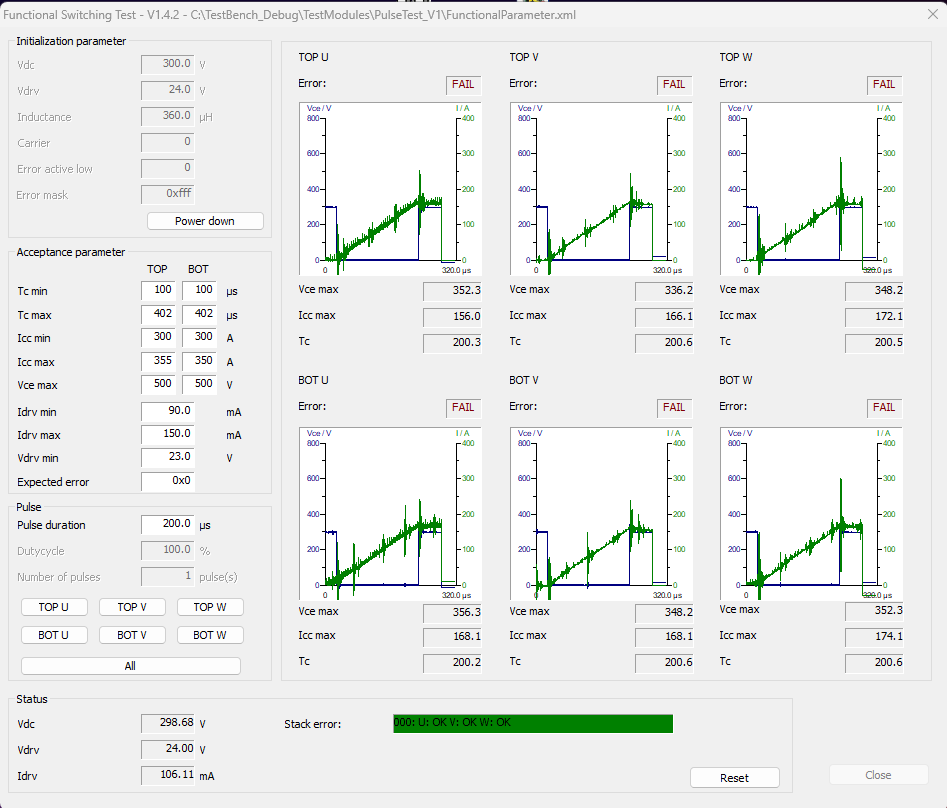
\includegraphics[width=0.8\textwidth]{Grafiken/Beispiel_Teststandgraphen}
    \caption{Beispiel der Graphen aus Teststandprogramm}
    \label{fig:2. Beispiel der Graphen aus Teststandprogramm}
    {Quelle: Eingenaufnahme}
\end{figure}